\documentclass[10pt,twocolumn,letterpaper]{article}

\usepackage{icb}
\usepackage{times}
\usepackage{epsfig}
\usepackage{graphicx}
\usepackage{amsmath}
\usepackage{amssymb}
\usepackage{listings}
\usepackage{url}

% Include other packages here, before hyperref.

% If you comment hyperref and then uncomment it, you should delete
% egpaper.aux before re-running latex.  (Or just hit 'q' on the first latex
% run, let it finish, and you should be clear).
%\usepackage[pagebackref=true,breaklinks=true,letterpaper=true,colorlinks,bookmarks=false]{hyperref}

\icbfinalcopy % *** Uncomment this line for the final submission

\def\icbPaperID{****} % *** Enter the IJCB Paper ID here
\def\httilde{\mbox{\tt\raisebox{-.5ex}{\symbol{126}}}}

% Pages are numbered in submission mode, and unnumbered in camera-ready
\ificbfinal\pagestyle{empty}\fi
\begin{document}

%%%%%%%%% TITLE
\title{A framework for Indoor Scene recognition}

\author{Thomas Bergmueller\\
Authentic Vision, University of Salzburg\\
Salzburg, Austria\\
{\tt\small tb@authenticvision.com}
% For a paper whose authors are all at the same institution,
% omit the following lines up until the closing ``}''.
% Additional authors and addresses can be added with ``\and'',
% just like the second author.
% To save space, use either the email address or home page, not both
\and
Eleftherios Christopoulos, Martin Schnoell\\
University of Salzburg\\
Salzburg, Austria\\
{\tt\small \{mschnoell, echristopoulos\}.aise-m2013@fh-salzburg.ac.at}
}

\maketitle
\thispagestyle{empty}

%%%%%%%%% ABSTRACT
\begin{abstract}
   The ABSTRACT is to be in fully-justified italicized text, at the top
   of the left-hand column, below the author and affiliation
   information. Use the word ``Abstract'' as the title, in 12-point
   Times, boldface type, centered relative to the column, initially
   capitalized. The abstract is to be in 10-point, single-spaced type.
   Leave two blank lines after the Abstract, then begin the main text.
   Look at previous ICB abstracts to get a feel for style and length.
\end{abstract}

%%%%%%%%% BODY TEXT
\section{Introduction}
TODO

\section{Data set}
\label{sec:data}
For testing, we employ the MIT indoor scene recognition database \cite{indoorScenes}. The authors in \cite{indoorScenes} already point out desireable results by comparing the performance of 
\begin{itemize}
	\item Visual words with SIFT-Features
	\item Gist features \cite{oliva06}, which is a content-based method and
	\item RGB-classification \cite{indoorScenes}, where mean RGB-images of the particular scenes were used for training.
\end{itemize}

Along the database, the authors ship two text files, one, \emph{TrainImages.txt}, listing the pre-selected training data and another one, \emph{TestImages.txt}, listing the pre-selected test data. We stick to this pre-defined splitting of the data set since this ensures comparability with results found in literature. The data set contains a total of 15620 images showing 67 indoor scene categories. The data is structured in folders, where each folder represents one scene category. Interestingly, although the authors claim in \cite{indoorScenes} that the data set using these pre-selection files is partitioned resulting in 80 training images and 20 per class, we observe that although the total number of files ($67*(20+80) = 6700$) is correct, some classes in training and testing have an unexpected number of files, e.g. 79 for training or 23 for testing. Despite that, we stick to the proposed selection for the sake of comparable results.

The structure of the data base allows to retrieve the ground truth, namely the category each image belongs to from the full path to a particular image. We employ an image processing pipeline, where we store results after each intermediate steps in a separate folder. Doing so, we take advantage of firstly being forced to create a sensible interface between the detection stages and secondly, we cut down on computation time in the development process when parts of just one step in the pipeline is changed. However, we change the labeling of the $C=67$ classes from alphanumeric to integer labeling to simplify processing with Matlab. Additionally, \cite{indoorScenes} suggests grouping into five large groups, Store, Home, Public spaces, leisure and Working place. We keep this as an option by training the SVM differently if need be, namely by mapping the class labels to the five categories.



\section{Processing pipeline}
In order to classify scenes, we use the processing pipeline shown in figure \ref{fig:pipeline}. We propose the following structure to store data for exchange between the different steps of the pipeline:


\begin{lstlisting}
{
	fv,
	targets,
	class
}
\end{lstlisting}

Each row in x, targets and class corresponds to one data set entry, i.e. an image in the data set. Hence, the contents are row-vectors. We denote accessing the $i^{th}$ entry (row) of an field of the data structure $d$ as $d.field(i)$. 

The targets-field contains the ground truth obtained from the data set's labelling. This is typically an integer number or string. The class-field contains the classifier-output, namely the decision the complete processing pipeline made. Therefore, the evaluation of the processing pipeline's performance on a test data set $d$ with $N \in \mathbb{N}$ images can easily be conducted by computing the rate of matches between targets and classification results (refer section \ref{sec:eval}).

The \emph{fv}-field of the structure corresponds to the actual content of a data set, subsequently denoted as \emph{feature fector FV}. This could be high- and low-level feature vectors or empty. Note that the length of the FV has to be consistent throughout the rows.


\begin{figure}
	\begin{center}
		

	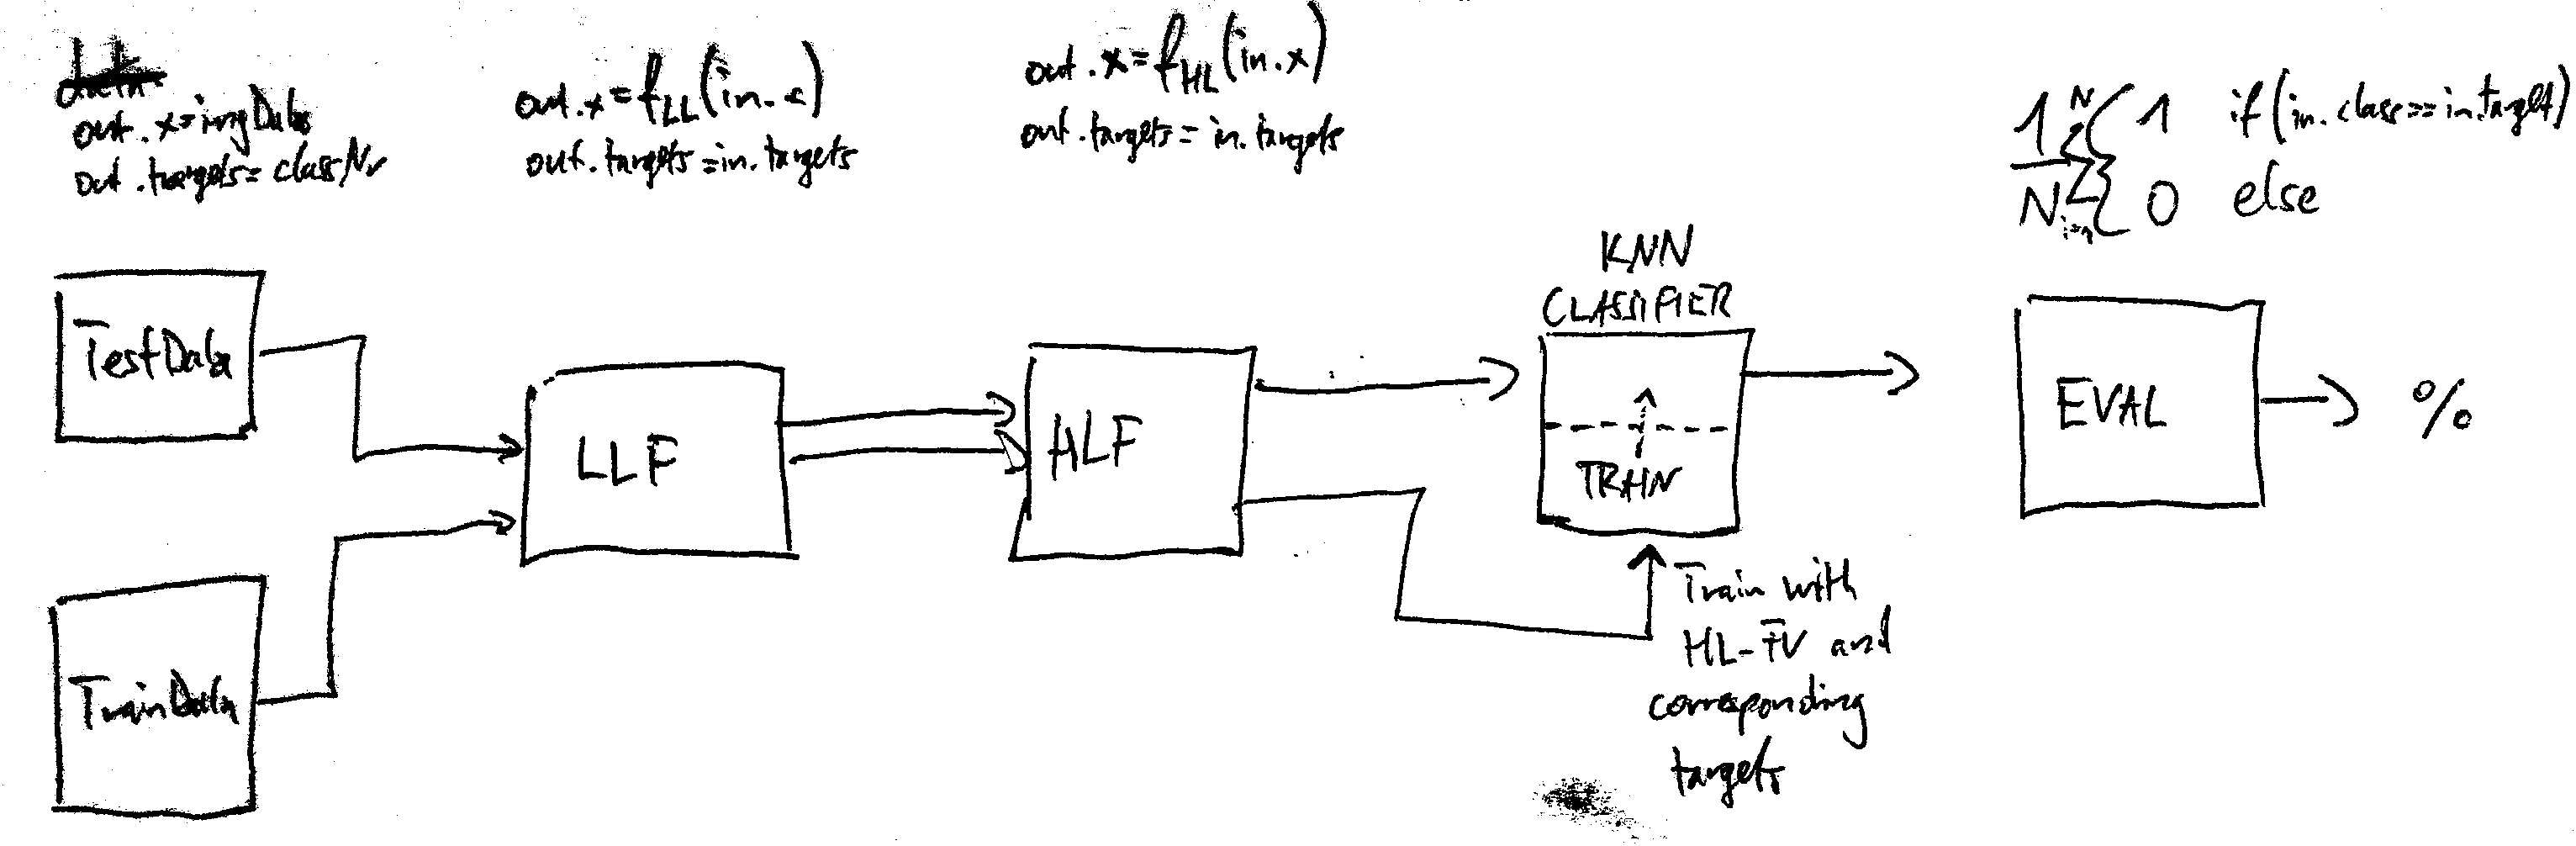
\includegraphics[width=\linewidth]{img/pipeline}
	\label{fig:pipeline}
	\caption{Processing pipeline of test- and training-data}
		\end{center}
\end{figure}


In the following sections we discuss and document the different steps of the processing pipeline, which is shown in figure \ref{fig:pipeline}.

\subsection{Low-level Feature Extraction}
The low-level feature extraction individually loads the images of the test- and training-data sets, which have been created as described in section \ref{sec:data}. As soon as the $i^{th}$ image $I^{(i)}$ is loaded, the low-level featureExtraction $f_{LL}$ is applied on this image and the result, which is a feature row-vector of fixed length $L_{LL}$, is assigned to the structured data set's feature vector. The ground truth, which is retrieved from the filename of the image (denoted as class($I^{(i)}$) is stored in the structure's targets. This process is denoted as 

\begin{small}

\begin{eqnarray}
d.fv(i) & = & f_{LL}(I^{(i)}) \quad \text{with} \quad f_{LL} \in \mathbb{R}^{1 \times L_{LL}} \\
d.targets(i)& = &class((I^{(i)})
\end{eqnarray}  

\end{small}

After this is done, the data is typically stored to the hard disk as Matlab .mat files. This has the advantage of avoiding to recompute the whole pipeline while developing a certain step of the processing pipeline. Besides Classification, Lowlevel feature extraction is usually the computationally most expensive part, because it processes the largest amount of data.
\subsection{High-level Feature Extraction}

Similar

\subsection{Classifier}
For classification, we use (as also in \cite{indoorScenes}) a support vector machine (SVM). The SVM is trained using the high-level features of the training data together with the class labelling retrieved from the targets, i.e. $mySVM.train(traindata.targets, traindata.fv)$. After training, $testdata.class$ is assigned the result of the prediction process $svm.predict(testdata.fv)$. 

Since SVMs are typically designed to solve two-class problems, we chose to use a MulticlassSVM. An implementation is available at Matlab's fileexchange\footnote{\url{http://www.mathworks.com/matlabcentral/fileexchange/39352-multi-class-svm}}. However, this implementation is really slow in training, especially for 67 classes. This is why we're looking for alternatives now.

\subsection{Evaluation}
\label{sec:eval}
Evaluation of the data is straight forward. It is simply evaluated, to which extent the SVM-classification lead to the correct results. That is, where the $i^{th}$ $d.class(i)$ matches the ground truth $d.targets(i)$. Formally, the recognition rate, namely the correctly classified scenes, can be computed as 
\begin{small}

\begin{equation}
	recognitionRate = \frac{1}{N} \sum_{i=1}^{N} \begin{cases}
	1 \quad \text{if} \quad d.targets(i) = d.class(i)\\
	0  \quad \text{else}
	\end{cases}
\end{equation}
\end{small}


Based on this processing pipeline, we evaluate different methods for Highlevel- and lowlevel feature extraction.

\section{Methods}

\subsection{Low-level features}

\subsection{High-level features}

\section{Results}

\section{Conclusion}


{\small
\bibliographystyle{ieee}
\bibliography{egbib}
}

\end{document}
